\documentclass[pstricks,14 pt]{extarticle}

	\usepackage[frenchb]{babel}
	\usepackage[utf8]{inputenc}  
	\usepackage[T1]{fontenc}
	\usepackage{amssymb}
	\usepackage[mathscr]{euscript}
	\usepackage{stmaryrd}
	\usepackage{amsmath}
	\usepackage{tabularx} 
	\usepackage{pstricks}
	\usepackage{pst-all} 
	\usepackage{tikz}
	\usepackage[all,cmtip]{xy}
	\usepackage{amsthm}
	\usepackage{varioref}
	\usepackage{geometry}
	\geometry{a4paper}
	\usepackage{lmodern}
	\usepackage{hyperref}
	\usepackage{array}
	 \usepackage{fancyhdr}
\usepackage{pstricks-add,multido}
	 \usepackage{float}
\renewcommand{\theenumi}{\alph{enumi})}
	\pagestyle{fancy}
	\theoremstyle{plain} 
	\fancyfoot[C]{} 
	\fancyhead[L]{Contrôle}
	\fancyhead[R]{Géométrie dans l'espace}\geometry{
 a4paper,
 total={170mm,287mm},
 left=10mm,
 right=10mm,
 top=8mm,
 bottom = 8mm
 }
	
	
	\title{Contrôle }
	\date{}
	\begin{document} 
\subsection*{Exercice 1 - 10 points}	%(1 + 2 + 2 + 1)  
Réduire les expressions suivantes : 
\begin{enumerate}
\item $(3x+1) + (x+3)$
\item $(3x+1)-(x+3)$
\item $x(2x-4)$
\item $(3x+1)(x+3)$
\end{enumerate}
Factoriser les expression suivantes : 
\begin{enumerate}
\item $3x + 9$
\item $5x^3 - 3x$
\item $(x+1)(x+2) - (x-3)(x+1)$
\end{enumerate}
Combien valent : \begin{enumerate}
\item un prix de $15$ euros après une augmentation de $10\%$.
\item le prix initial d'un objet valant $36$ euros après avoir augmenté de
$20\%$. 
\item le prix initial d'un billet valant $64$ euros après une réduction de $20\%$.
\end{enumerate} 

\subsection*{Exercice 2 - 10 points}	%(1 + 2 + 2 + 1)  
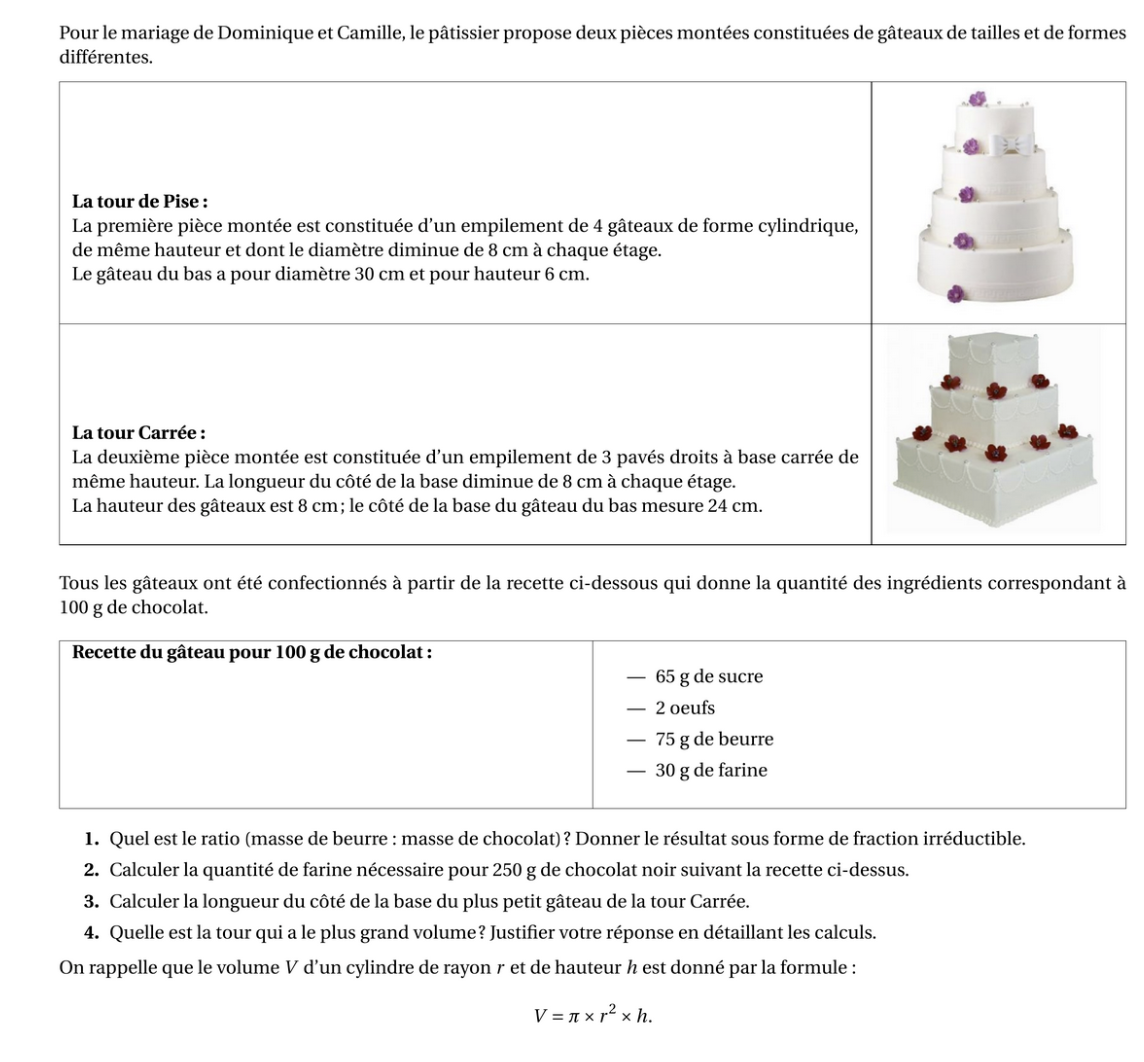
\includegraphics[scale=.85]{Probleme}
 	\end{document}
